%Evaluation
\section{Evaluation}
\label{sec:eval}
Finally, we must judge our system's performance directly, to demonstrate the effectiveness of our ideas in practice.
\subsection{Metrics}
\label{subsec:metrics}
In order to judge the usefulness of our system, we need some way to compute how well \bitr\ reconstructed types on a known compilation. Previous work usually split accuracy and conservatism into separate measures~\cite{tie,sw}. Conservatism here is usually done as a measurement of how often inference is wrong, whether due to a bug or an inherent problem with the system. There have been many different approaches to accuracy measurement. TIE~\cite{tie} used a distance metric based on lattice distance, with inner portions of the type counting less for accuracy. SecondWrite~\cite{sw} reforms this somewhat, defining their pointer recovery accuracy based on detecting the number of indirections. However, their modification still leaves the question of how to evaluate structure correctness unaddressed. REWARDS~\cite{rewards}, as a dynamic system, did take into account the layers of indirection, as REWARDS categorized memory locations in the image. However, REWARDS used a simple notion of correctness, checking whether the types presented for a given piece of memory were equal to the debug type in its entirety.

In addition to the differing notions of accuracy and what correct means, there is an issue with the decoupling of the conservatism, accuracy, and precision metrics. When decoupled, non-conservatism resulting in greater apparent accuracy and precision is not necessarily punished in accordance with which type variables non-conservatism occurs on.

Additionally, lattice distance is not a great measurement of accuracy, as simply guessing that all variables are integers of size equal to their storage size is effective on the distance scale. Many variables are integers, and integers are only a short distance away from the pointer type if the type turns out to be pointer-sized, and this is directly at the middle of the top to bottom range. The lattice model further falls apart when we consider the notion of alternative lattices. When comparing two systems, which lattice should measure the distance between types on? Are two systems even comparable anymore? As more work occurs in type reconstruction, having a metric which will allow for the comparison of systems with radically different views of typing will be important.

We mix the notions of accuracy, conservatism, and precision together into a single metric. We define as our quality metric over a binary:
\[
Q = E[B(A) \in C(A)] = \frac{1}{n}\sum_{A} \frac{|C(A) \cap B(A)|}{|B(A)|}
\]
where $B(A)$ is the set of types \bitr\ recommends for type variable $A$, and $C$ the set of types (usually a singleton) given by debugging information or ground truth.

This has a slight abuse of notation. Within the expected value, $B(A)$ is a random variable that generates a uniformly random member of the set $B(A)$. Additionally, in the expected value, $A$ is the random variable picking a uniformly random value from the domain of $C$

This metric represents the rate at which a user of the system would be correct if it selected a type uniformly from our recommendations. This kind of evaluation represents the expected performance in an environment similar to what a user might experience if reverse engineering code --- each time they ask the system for assistance, what is the probability that the system will recover the relevant portion of the debugging information.

Unfortunately, we can only compare ourselves to TIE with this metric, as we do not have access to implementations of the other systems. Note that while TIE describes a methodology for comparing its results against structure types, it does not in practice actually produce structure types. We report conservativeness and average lattice distance as well, but we do not consider these our primary objectives.

%  List of questions, each corresponding to a subsection
\subsection{Can \bitr\ recover types in sample cases?}
In small example programs which sum lists, walk binary trees, and perform simple look-ups in arrays of structs, we achieved 100\% success. They provide a stark comparison to TIE, which produced 11\% on summation of lists (corresponding to all things of a given size being valid), correctly identified the temporary variables in the tree walking for 15\%, and could not determine that the global array containing the structs in existed, getting another 12\% on temporary variables. We mention these programs to highlight that \bitr\ handles behavior that was previously not even measured in the literature. Hex-Rays'~\cite{ida} performance on the loop summation example, as seen in the introduction, would have scored a 14\% with that output. Note that the comparison here is somewhat unfair, because IDA must express exactly one type to the user. As a result, Hex-Rays' other numbers are not reported as the comparison is not meaningful or fair.

\subsection{Does \bitr's recovery ability exceed previous work?}
\label{subsec:evalprev}
\begin{figure*}
\centering{
\begin{tabular}{|c||c|c|c|}
\hline
Implementation & Unconstrained & Constrained & Conservativity \\
\hline
\bitr & $21.02\% \pm 2.64$ & $38.00\% \pm 5.81$ & $91.72\% \pm 3.35$\\
TIE & $12.64\% \pm 7.06$ & $16.80\% \pm 1.63$ & $90.31\% \pm 2.66$\\
\hline
\hline
Improvement & 8.38\% & 21.2\% & 1.41\%\\
\hline
\end{tabular}
}
\caption{Result Summary (Probability Metric)}
\label{bitr:fig:results-prob}
\end{figure*}
\begin{figure*}
\centering{
\begin{tabular}{|c||c|c|}
\hline
	Implementation & Unconstrained Dist. & Constrained Dist.\\
\hline
\bitr & $1.32 \pm 0.06$ & $0.65 \pm 0.075$\\
TIE & $2.10 \pm 0.044$ & $1.58 \pm 0.25$\\
\hline
\hline
Improvement & 0.78 & 0.93 \\
\hline
\end{tabular}
}
\caption{Result Summary (TIE Distance Metric)}
\label{bitr:fig:results-tie}
\end{figure*}

For a more real-world evaluation, we ran our system and TIE~\cite{tie} with our new metric, over \texttt{coreutils}, a collection of common programs installed on nearly every UNIX system. The programs in \texttt{coreutils} represent a variety of different kinds of workloads, and are open source, so we were readily able to build and examine debug symbols for them. We use this data set to answer this and our remaining questions.

In an effort to demonstrate the validity of our new metric and compare ourselves to systems other than TIE (on which we were able to generate our new metric scoring due to TIE access), we also report statistics of conservatism and distance in the same way as previous work~\cite{tie,sw}. Overall, on \texttt{coreutils} we achieve conservatism of 95.95\% and an average distance of only 1.33. If we only examine type variables which had at least one constraint reference them, we see instead an average distance of 0.68, substantially better than previous work.

\subsection{Is \bitr's recovery good on an absolute scale?}
Unfortunately, we cannot run most of the other systems under this metric, as implementations are not readily available. However, we did get access to an implementation of TIE, so we ran TIE under this new metric in addition to our work. Over all the type information contained in the DWARF information for \texttt{coreutils}, \bitr\ got a 21.01\% recovery rate. TIE, when scored on this metric, achieves a 12.65\% rate.

As our new metric has a direct interpretation in terms of its usefulness to the reverse engineer, these values show that \bitr\ is useful for recovering types. Additionally, it highlights the progress made on an absolute scale. However, it also shows how much further the field has to go --- a one in five chance of having the correct type is unlikely to be the best possible solution.

\noindent {\bf Under-constrained Types.}
One of the biggest sources of error in our analysis is under-constrained types. The code references and operates on these variables, but due to the low number of operations performed on them, there is no way to know definitively what the type of these variables are. For example, in the C snippet
\begin{verbatim}
int f(void* x) {
  ? v = x;
  return (v == 0);
}
\end{verbatim}
we would get code which would be legal if our mystery type were either an \texttt{int} or a pointer of some variety. We can use heuristics when outputting a type for decompilation (for example, preferring the lower bound of a type in order to avoid casting), but since both are legal, and all constraints on \texttt{v} are visible in this snippet, we would never be able to get an exact type.

Dealing with these would be a matter of better heuristics, and would have left the realm of program analysis and gone into the realm of programmer analysis. The heuristic of selecting the lower bound is not a good one, as this will reduce your conservativeness, but sometimes this choice may make sense. Developing heuristics to deal with this issue is outside the scope of this work, but presents an interesting challenge discovered in our experiments.

\subsection{How does \bitr\ fare at recovering constrained types?}
\begin{figure}
	\begin{center}
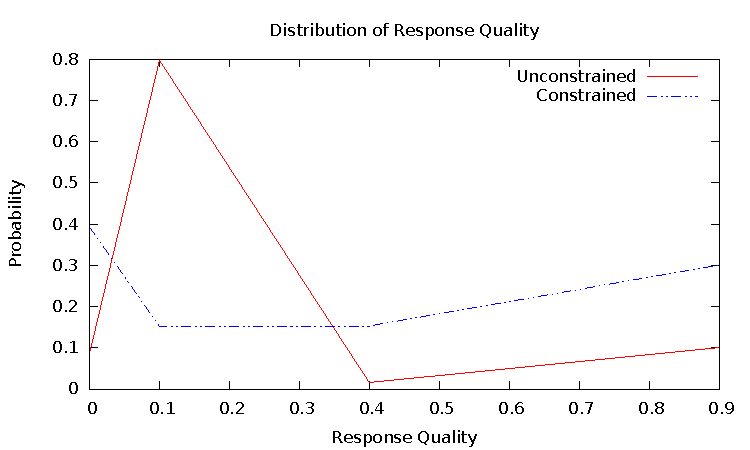
\includegraphics[scale=1.1]{bitr/quality.pdf}
	\end{center}
\caption{Effects of Unconstrained Type Variables}
\label{fig:unconst}
\end{figure}

In order to more closely examine the effect that unconstrained type variables have on our metrics, we generated a probability mass plot of response quality in both situations, as shown in Figure~\ref{fig:unconst}. This shows the
difference between responses that \bitr\ has constraints on, and those it does not.
When we restrict ourselves to type variables which the code accessed, causing a constraint to be generated, our recovery rate spikes to 36.78\%, showing great overall improvement.

This makes sense as a measurement because it demonstrates the ability of the tool to police the boundaries of its own knowledge. Specifically, it measures the performance of the tool when used as an advisor rather than as the sole source of types. When \bitr\ has seen the type variable in question constrained, it has a much greater level of information available on what the type could be.

\noindent {\bf Unconstrained Type Variables.}
The primary source of error reflected in this difference is data that is never written to or read from. For example, while most \texttt{coreutils} binaries contain a \texttt{close\_stream} function which operates on a stream structure, there is no indication of the inner properties of this structure in the code itself. However, the debug symbols are constructed in the presence of header files that describe the fields of the stream structure. As a result, the score is strongly deflated.
We can partially mitigate this by using type signatures for library functions, but we did not use signatures for all functions in our experiments, nor would this information always be available.
While \bitr\ can recover some of these unconstrained variables through appropriate type signing (or analysis of the target shared library), there are also a cases where a structure is present, but in the structure's entire life cycle, one of its fields is never referenced.

\subsection{How does \bitr\ scale?}
\label{subsec:speed}
It is important to note its scaling characteristics relative to the size of the input problem. Two good proxies for problem size are number of type variables and number of constraints. In practice, in our conjunction of disjunctions, there are about approximately as many disjunctive clauses as there are type variables. \bitr\ experimentally uses an amount of memory linear in both of number of constraints and type variable count, and time proportional to the square. This happens because when checking consistency, the system checks each live type variable rather than only those whose constraints may have changed. Adding an optimization which only checked those type variables affected directly or indirectly by incorporating a new constraint would be expected to replace a factor of $N$ with $K \log N$ by removing the requirement to check every live type variable.
